        \documentclass{article}
        \usepackage[margin=1in]{geometry}
        \usepackage{hyperref}
        \usepackage{amsmath,amsfonts,amssymb,amsthm,commath,dsfont}
        \usepackage{enumitem}
        \usepackage{bbold}
        \usepackage{amsmath}
        \usepackage{framed}
        \usepackage{xspace}
        \usepackage{booktabs}
        \usepackage{microtype}
        \usepackage{float}
        \usepackage[round]{natbib}
        \usepackage{cleveref}
        \usepackage[dvipsnames]{xcolor}
        \usepackage{graphicx}
        \usepackage{listings}
        \usepackage[breakable]{tcolorbox}
        \tcbset{breakable}
        \usepackage{bbm}
        \usepackage{mathtools}
        %\usepackage{symbols}
        \usepackage{subcaption}
        
        \usepackage{pifont}
        \newcommand{\cmark}{\ding{51}}
        \newcommand{\xmark}{\ding{55}}
        \newcommand{\vect}[1]{\boldsymbol{#1}}
        \newcommand{\colbar}{\rule[-3mm]{.3mm}{1.5em}}
        \newcommand{\rowbar}{\rule[.5ex]{1.5em}{.3mm}}
        \DeclareMathOperator{\rank}{rank}
        \DeclareMathOperator*{\argmax}{argmax}
        \DeclareMathOperator*{\argmin}{argmin}

        % following loops stolen from djhsu
        \def\ddefloop#1{\ifx\ddefloop#1\else\ddef{#1}\expandafter\ddefloop\fi}
        % \bbA, \bbB, ...
        \def\ddef#1{\expandafter\def\csname bb#1\endcsname{\ensuremath{\mathbb{#1}}}}
        \ddefloop ABCDEFGHIJKLMNOPQRSTUVWXYZ\ddefloop
        
        % \cA, \cB, ...
        \def\ddef#1{\expandafter\def\csname c#1\endcsname{\ensuremath{\mathcal{#1}}}}
        \ddefloop ABCDEFGHIJKLMNOPQRSTUVWXYZ\ddefloop
        
        % \vA, \vB, ..., \va, \vb, ...
        \def\ddef#1{\expandafter\def\csname v#1\endcsname{\ensuremath{\boldsymbol{#1}}}}
        \ddefloop ABCDEFGHIJKLMNOPQRSTUVWXYZabcdefghijklmnopqrstuvwxyz\ddefloop
        
        % \valpha, \vbeta, ...,  \vGamma, \vDelta, ...,
        \def\ddef#1{\expandafter\def\csname v#1\endcsname{\ensuremath{\boldsymbol{\csname #1\endcsname}}}}
        \ddefloop {alpha}{beta}{gamma}{delta}{epsilon}{varepsilon}{zeta}{eta}{theta}{vartheta}{iota}{kappa}{lambda}{mu}{nu}{xi}{pi}{varpi}{rho}{varrho}{sigma}{varsigma}{tau}{upsilon}{phi}{varphi}{chi}{psi}{omega}{Gamma}{Delta}{Theta}{Lambda}{Xi}{Pi}{Sigma}{varSigma}{Upsilon}{Phi}{Psi}{Omega}{ell}\ddefloop

        \newcommand\T{{\scriptscriptstyle\mathsf{T}}}
        \def\diag{\textup{diag}}
        
      

        \def\SPAN{\textup{span}}
        \def\tu{\textup{u}}
        \def\R{\mathbb{R}}
        \def\E{\mathbb{E}}
        \def\Z{\mathbb{Z}}
        \def\be{\mathbf{e}}
        \def\nf{\nabla f}
        \def\veps{\varepsilon}
        \def\cl{\textup{cl}}
        \def\inte{\textup{int}}
        \def\dom{\textup{dom}}
        \def\Rad{\textup{Rad}}
        \def\lsq{\ell_{\textup{sq}}}
        \def\hcR{\widehat{\cR}}
        \def\hcRl{\hcR_\ell}
        \def\cRl{\cR_\ell}
        \def\hcE{\widehat{\cE}}
        \def\cEl{\cE_\ell}
        \def\hcEl{\hcE_\ell}
        \def\eps{\epsilon}
        \def\1{\mathds{1}}
        \newcommand{\red}[1]{{\color{red} #1}}
        \newcommand{\blue}[1]{{\color{blue} #1}}
        \def\srelu{\sigma_{\textup{r}}}
        \def\vsrelu{\vec{\sigma_{\textup{r}}}}
        \def\vol{\textup{vol}}

        \newcommand{\ip}[2]{\left\langle #1, #2 \right \rangle}
        \newcommand{\mjt}[1]{{\color{blue}\emph\textbf{[M:}~#1~\textbf{]}}}
        \newcommand{\sahand}[1]{{\color{green}\emph\textbf{[Sah:}~#1~\textbf{]}}}
		
        \newtheorem{fact}{Fact}
        \newtheorem{lemma}{Lemma}
        \newtheorem{condition}{Condition}
        \theoremstyle{definition}
        \theoremstyle{remark}
        \newtheorem{remark}{Remark}
        \newtheorem{example}{Example}

        \newenvironment{Q}
        {%
          \clearpage
          \item
        }
        %{%
       %   \phantom{s} %lol doesn't work
       %     \bigskip
        %    \textbf{Solution.}
        %  }

        \title{CS 446 / ECE 449 --- Homework 4}
        \author{\emph{your NetID here}}
        \date{Version 1.0}

        \begin{document}
        \maketitle

        \noindent\textbf{Instructions.}
        \begin{itemize}
          \item
            Homework is due \textbf{Tuesday, April 6th, at noon CST}; no late homework accepted.
        
          \item
            Everyone must submit individually at gradescope under \texttt{hw4} and \texttt{hw4code}.
        
          \item
            The ``written'' submission at \texttt{hw4} \textbf{must be typed}, and submitted in
            any format gradescope accepts (to be safe, submit a PDF).  You may use \LaTeX, markdown,
            google docs, MS word, whatever you like; but it must be typed!
        
          \item
            When submitting at \texttt{hw4}, gradescope will ask you to mark out boxes
            around each of your answers; please do this precisely!
        
          \item
            Please make sure your NetID is clear and large on the first page of the homework.
        
          \item
            Your solution \textbf{must} be written in your own words.
            Please see the course webpage for full academic integrity information.
            Briefly, you may have high-level discussions with at most 3 classmates,
            whose NetIDs you should place on the first page of your solutions,
            and you should cite any external reference you use; despite all this,
            your solution must be written in your own words.
        
          \item
            We reserve the right to reduce the auto-graded score for
            \texttt{hw4code} if we detect funny business (e.g., your solution
            lacks any algorithm and hard-codes answers you obtained from
            someone else, or simply via trial-and-error with the autograder).
            
          \item
           When submitting to \texttt{hw4code}, only upload \texttt{hw4.py} and \texttt{hw4\_utils.py}. Additional files will be ignored.
        
        \end{itemize}
        
       
       \begin{enumerate}[font={\Large\bfseries},left=0pt]
	   \begin{Q}
\textbf{\Large Principal Component Analysis}\\

\begin{enumerate}

\item For each of the following statements, specify whether the statement is true or false. If you think the statement is wrong, explain in 1 to 2 sentences why it is wrong.


\begin{itemize}
\item True or False: As shown in the figure below, PCA seeks a subspace such that the sum of all the vertical distance to the subspace (the dashed line) is minimized.
\begin{center}
 \includegraphics[width=8cm]{figs/pca.pdf}
 \end{center}

\item True or False: PCA seeks a projection that best represents the data in a least-squares sense.

\item  True or False: PCA seeks a linear combination of variables such that the maximum variance is extracted from the variables. 

\item True or False: The principal components are not necessarily orthogonal to each other. \\

\item True or False: Solving PCA using SVD might result in a solution which corresponds to a local minimum.
\end{itemize}


\item Recall that PCA finds a direction $w$ in which the projected data has highest variance by solving the following program:
	\begin{equation}
	\max_{w:||w||^2=1}w^T\Sigma w.
	\label{equ:pca}
	\end{equation}
	Here, $\Sigma$ is a covariance matrix. You are given a dataset of two 2-dimensional points $(1,3)$ and $(4,7)$. Draw the two data points on the 2D plane. What is the first principal component $w$ of this dataset?

\item Now you are given a dataset of four points $(2,0)$, $(2,2)$, $(6,0)$ and $(6,2)$. Draw the four data points on the 2D plane. Given this dataset, what is the dimension of the covariance matrix $\Sigma$ in Eq.~\eqref{equ:pca}? Also, explicitly write down the values of $\Sigma$ given the dataset.

\item What is the optimal $w$ and the optimal value of the program in Eq.~\eqref{equ:pca}  given \[ \Sigma= \left[ \begin{array}{cccc}
	12 & 0 & 0 & 0\\
	0 & 6 & 0 & 0\\
	0 & 0 & 20 & 0\\
	0 & 0 & 0 & 10\\
	\end{array} \right]\] 


\end{enumerate}
\end{Q}
                  
	   %\input{pca_sol.tex}             
       
        \begin{Q}
\textbf{\Large Gaussian Mixture Models}\\

Consider a Gaussian mixture model with $K$ components ($k\in\{1, \ldots, K\}$), each having mean $\mu_k$, variance $\sigma_k^2$, and mixture weight $\pi_k$. Further, we are given a dataset $\mathcal{D} = \{x_i\}$, where $x_i \in \mathbb{R}$. We use $z_{i} = \{z_{ik}\}$ to denote the latent variables.


\begin{enumerate}

\item What is the log-likelihood of the data according to the Gaussian Mixture Model? (use $\mu_k$, $\sigma_k$, $\pi_k$, $K$, $x_i$, and $\mathcal{D}$).

\item Assume $K=1$,  find the maximum likelihood estimate for the parameters ($\mu_{1}$, $\sigma_{1}^{2}$, $\pi_{1}$).

\item What is the probability distribution on the latent variables, i.e., what is the distribution
$p(z_{i,1}, z_{i,2}, \cdots, z_{i,K} )$ underlying Gaussian mixture models. Also give its name.


\item For general $K$, what is the posterior probability $p(z_{ik} = 1|x_i)$? To simplify, wherever possible, use $\mathcal{N}(x_{i}|\mu_{k},\sigma_{k})$, a Gaussian distribution over $x_{i} \in \mathbb{R}$ having mean $\mu_{k}$ and variance $\sigma_{k}^2$.


\item  How are k-Means and Gaussian Mixture Model related? (There are three conditions)

\item Consider the modified Gaussian Mixture Model objective:
$$
\min_{\mu} - \sum_{x_{i} \in \mathcal{D}} \epsilon \log \sum_{k=1}^{K} \exp{(-(x_{i} - \mu_{k} )^{2}/\epsilon) }.
$$
We denote by $F_{k}= (x-\mu_{k})^{2}$. Show that:
$$
\lim_{\epsilon \rightarrow 0} \epsilon \log \sum_{k=1}^{K} \exp{(-F_{k}/\epsilon) } = \sum_{k=1}^{K}  \mathbb{1}_{\{k=\argmin\limits_{k} F_{k}  \}} F_{k}, \quad \epsilon \in \mathbb{R}^{+}
$$
\textbf{Hint:} Use l'Hopital rule.

\item Conclude that the objective for k-Means is the 0-temperature limit of Gaussian Mixture Model under the conditions you provided in part (e).


\end{enumerate}

\end{Q}
                  
	  %\input{gmm_sol.tex}
	    
	   \input{EM.tex}        
	   %\input{EM_sol.tex}  
	   
	 \begin{Q}
\textbf{\Large K-Means 1}\\

\begin{enumerate}

\item Mention if K-Means is a supervised or an un-supervised method and state the reason.

\item Assume that you are trying to cluster data points $x_{i}$  for $ i \in \{1,2, \dots, D\}$ into $K$ clusters each with center $\mu_{k}$  where $ k \in \{1,2, \dots, K \}$. The objective function for doing this clustering involves minimize the euclidean distance between the points and the cluster centers. It is given by  \begin{equation*}
\min\limits_{\mu} \min\limits_{r}\sum\limits_{i \in D} \sum\limits_{k =1}^{K} \frac{1}{2} r_{ik} \|x_{i} -\mu_{k}\|_{2}^{2}. \\
 \end{equation*} \\ How do you ensure hard assignment of one data point to one and only one cluster at a given time?
 
 \textbf{Hint:} By hard assignment we mean that you are 100 \% sure that a point either belongs or doesn't belong to a cluster.
 
 \item How does your answer to part b change if we want to obtain a soft assignment instead?
 
 \textbf{Hint:} By soft assignment we mean that  a point  belongs to a cluster with some probability.
 
 \item Looking at the following plot, what is the best choice for the number of clusters?
 \begin{center}
 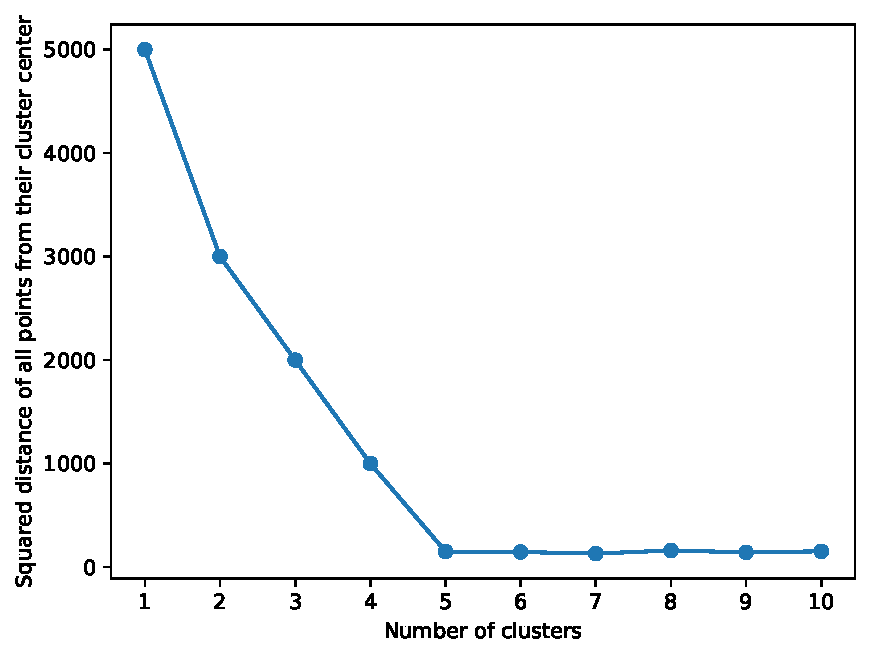
\includegraphics[width=8cm]{figs/cluster.pdf}
 \end{center}
 
 \item Would K-Means be an efficient algorithm to cluster the following data? Explain your answer in a couple of lines.
 \begin{center}
 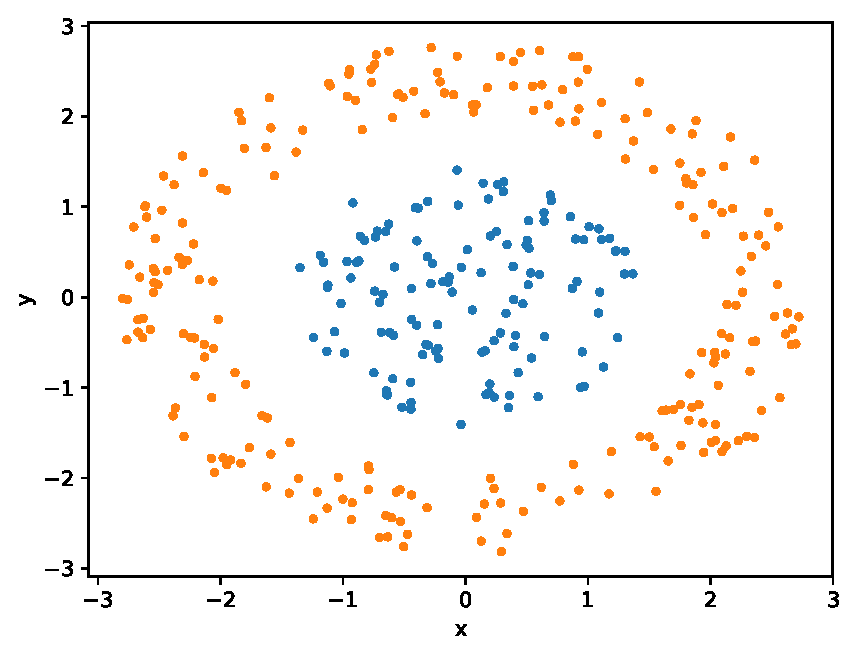
\includegraphics[width=8cm]{figs/concentric.pdf}
 \end{center}

\end{enumerate}


\end{Q}
                  
	  %\input{kmeans1_sol.tex}     
	  
	  \begin{Q}
\textbf{\Large K-Means 2}\\

We are given a dataset $\cD = \{(x)\}$ of 2d points $x\in\mathbb{R}^2$ which we are interested in partitioning into $K$ clusters, each having a cluster center $\mu_k$ ($k\in\{1, \ldots, K\}$) via the $k$-Means algorithm. This algorithm optimizes the following cost function:
\begin{equation}
	\min_{\mu_k, r} \sum_{x\in\cD,k\in\{1, \ldots, K\}} \frac{1}{2}r_{x,k}\|x - \mu_k\|_2^2 \quad\quad\text{s.t.}\quad \left\{\begin{array}{ll}
r_{x,k}\in\{0,1\}&\forall x\in\cD,k\in\{1, \ldots, K\}\\
\sum_{k\in\{1, \ldots, K\}} r_{x,k} = 1 & \forall x\in\cD
\end{array}\right.
\label{eq:KMeans2:main}
\end{equation}

\begin{enumerate}

\item What is the domain for $\mu_k$?

\item Given fixed cluster centers $\mu_k$ $\forall k\in\{1, \ldots, K\}$, what is the optimal $r_{x,k}$ for the program in Eq. \ref{eq:KMeans2:main}? Provide a reason?

\item Given fixed $r_{x,k}$ $\forall x\in\cD,k\in\{1, \ldots, K\}$, what are the optimal cluster centers $\mu_k$ $\forall k\in\{1, \ldots, K\}$ for the program in Eq. \ref{eq:KMeans2:main}? 

\textbf{Hint:} Reason by first computing the derivative w.r.t $\mu_k$.

\item Using Pseudo-code, sketch the algorithm which alternates the aforementioned two steps. Is this algorithm guaranteed to converge and why? Is this algorithm guaranteed to find the global optimum? What is the reason?

\textbf{Hint:} you can provide a counter-example to invalidate a statement.

\item Please implement the aforementioned two steps. For the given dataset, after how many updates does the algorithm converge, what cost function value does it converge to and what are the obtained cluster centers? Visualize clusters at each step and attach the plots here. Please at least report numbers with one decimal point.

\textbf{Remark:} how we count updates: when computing a set of new centroids from initilization, we call this one update.

\textbf{Hint:} You may find \texttt{hw4\_utils.vis\_cluster} useful.


\end{enumerate}


\end{Q}
                  
	 % \input{kmeans2_sol.tex}     
 
    \end{enumerate}
\end{document}
